% ============================================================
%  Figure — Per-sub-module W_err ablation for Stage 2 (Innovation-2)
%  FR-SVD (full) vs FR-SVD without Stage 2 (Stage-1-only) on LLaMA-7B
%  at 20% compression. Heatmap + module-wise bar chart.
%  Required preamble packages:
%    \usepackage{graphicx}
% ============================================================

\begin{figure}[t]
\centering
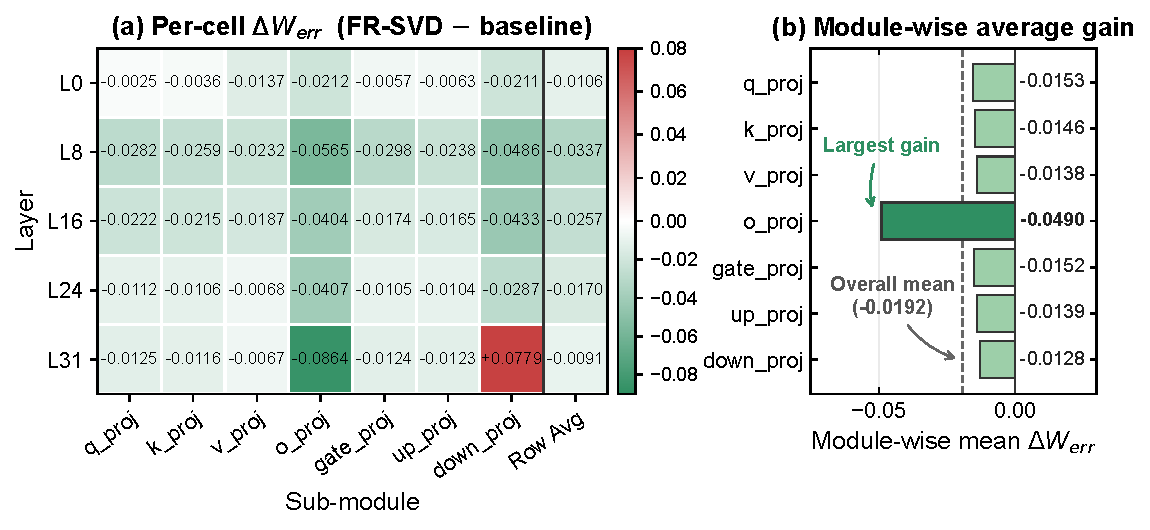
\includegraphics[width=\linewidth, trim=2 2 2 2, clip]{figs/figure_werr_submodule_ablation.pdf}
\caption{Submodule ablation of Stage~2 (eigenspace residual compensation)
on LLaMA-7B at $20\%$ compression on WikiText-2, showing the per-cell
$\Delta W_{\mathrm{err}}$ of FR-SVD relative to a Stage-1-only baseline
(i.e., FR-SVD without Stage~2). \textbf{(a)} Heatmap of
$\Delta W_{\mathrm{err}}$ over $5$ sampled layers
($L_{0}/L_{8}/L_{16}/L_{24}/L_{31}$) and $7$ submodules
(q/k/v/o/gate/up/down); the rightmost column reports the per-layer average.
Green denotes a reduction (FR-SVD better); red denotes an increase.
\textbf{(b)} Module-wise mean of $\Delta W_{\mathrm{err}}$ aggregated across
the five sampled layers; the dashed line marks the overall mean. The single
positive cell at $L_{31}$ \texttt{down\_proj} corresponds to a numerical
fallback artifact in the Stage-1-only baseline pipeline.}
\label{fig:werr-submodule-ablation}
\end{figure}
